\documentclass[Report.tex]{subfiles}
\externaldocument[I-]{chapter_1_introduction}
\externaldocument[D-]{chapter_3_discardMethod}
\externaldocument[R-]{chapter_4_result}
\externaldocument[C-]{chapter_5_conclusion}
\externaldocument[RE-]{chapter_6_recognition}


\begin{document}
\chapter{Method}
\label{sec:Method}
\section{Description}
The following section as described in Section~\ref{subsec:Report Layout} will
present our methods. Bellow we present each component individually and the
corresponding methods for them. A short description on what challenges have to
be solved for each component will be addressed first. \\ \\


\section{Component: Text segmentation}
\label{Method:Text_segmentation}

\subsection{Description}
In this part of the program, we want to be able segment out parts of text in the image. We want to then later segment out lines and letter for further classification. In this part wee assume that the image will mainly black text on white paper.

\subsection{Tried}
We where uncertain on how to do this part when we initial started the project. We ended up looking for a lot of different ways to do this part. We ended up trying 3 different approaches with mix result.
\begin{enumerate}
  \item Simple image analysis techniques, using Otsu thresholding and Morphology.(Used)
  \item Stroke Width Transform(SWT) to detect text in natural images.(Discarded)
  \item OpenCV implementation of Scene Text Detection.(Discarded)
\end{enumerate}

\begin{flushleft}
  \subsubsection{Approach 1: Simple Image Analysis Techniques}
  We was inspired by the this online blog \href{https://www.danvk.org/2015/01/07/finding-blocks-of-text-in-an-image-using-python-opencv-and-numpy.html}{Source}\cite{_finding_????}. We simplified the original approach to the following steps:
  \begin{enumerate}
    \item \textbf{Find Edges/Outliners of the image.}
    Initial idea is to use Canny, but we found Morphological Gradient to perform better. It indicates the contrast of the edges, so we can get better differences in some natural images.(so long the text and background is close to black and white)
    \item \textbf{Otsu Thresholding.}
    We need our image to be a binary image. We simply use OpenCV Otsu algorithm to achieve it.
    \item \textbf{Morphological Closing.}
    Since we want line segments we used Morphological Closing with large horizontal filter to merge as many horizontal letter together as possible.
    \item \textbf{Extract Regions}
    OpenCv FindContours was used to find the different text regions. We then exclude any regions that is smaller than a selected threshold. The different region are return as coordinate of the different rectangular boxes.
  \end{enumerate}
\end{flushleft}

\begin{flushleft}
  \subsubsection{Approach 2: Stroke Width Transform}
  The second approach we tried Stroke Width Transform to do Text Segmentation, it was original propose by Epstein et al 2010 \cite{epshtein_stroke_2010}. Since OpenCv do not have this implemented we tried to implement it ourself. Additional sources was used in our attempt to implement it\cite{werner_text_????, _c++_????, bunn_strokewidthtransform:_2018}. We was not able to finish this, but think we should mention it since we spend some time on it. The steps of Stroke Width Transform is as followed:
  \begin{enumerate}
    \item \textbf{Edge Detection and edge orientation(Done)}
    We need to have Edge image and orientation of the gradient image.
    Canny and Sobel was used in the original paper and other sources. This is simple since OpenCv have both Canny and Sobel implemented.
    \item \textbf{Stroke Width Transform(Done)}
    Here we had to do more. We have to find a line from a starting point and the angle. We was able to implement this part, but was some uncertainties. It only work on black text with white background. That is because the orientation(Sobel filtering) are dependent on it. The paper talk about doing a second pass with inverse image, but we decided to ignore it, in order to come farther in the algorithm.
    \item \textbf{Find Connected Component(Done)}
    In this point we are to connect component with the same Stride length together. We used One component at a time algorithm to find all the different components. We was able to finish it.
    \item \textbf{Exclude noise and find letters(not Done)}
    Since Stroke Width Transform tend to make a lot of noise. The obvious one is making single lines. This part are suppose to exclude this noise and at the same time exclude anything that is not a letter.The theory is, since letter and text all usually have the same stroke width, we can use this information do estimate what is letter and what is not. We was not able to finish this part.
    \item \textbf{Find lines/words(not Done)}
    Was not able to get to this part, but ideal it will combine letters to a single line or words.
  \end{enumerate}
  In cases where the image have a lot of non text object, it will work fine with it. We ended up discarding this approach since it was to time consuming and decided on working on simple approach first.
\end{flushleft}

\begin{flushleft}
  \subsubsection{Approach 3: OpenCv Scene Text Detection}
  OpenCV have it own Text Scene Detection. The approach of this algorithm is to detect text in scene using Classifier and Components Tree, propose by Lukás Neumann \& Jiri Matas \cite{neumann_real-time_2012}. Since we already discarded Stroke Width Transform to focus on simple approach, we decided not use it. We had some problem to get propel result as well.
\end{flushleft}

\subsection{Used in end result}
Since we had problem on getting with both approach 2 and 3 we decided on approach 1. It gave us ideal result on most images, but have some problem in images with non text objects.

\todo{fill the figure with good examples}
\begin{figure}[h]
  \centering
  \begin{subfigure}[t]{4cm}
    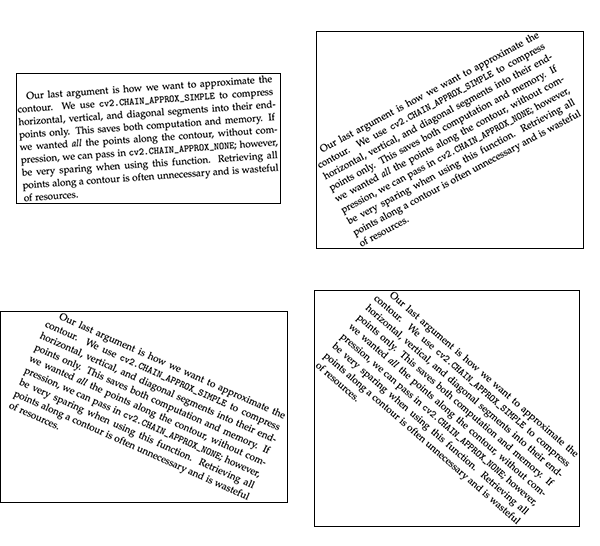
\includegraphics[width=3cm]{res/segment_text1.png}
    \caption{Example 1, Good result on just text}
  \end{subfigure}
  \hspace{5mm}%
  \begin{subfigure}[t]{4cm}
    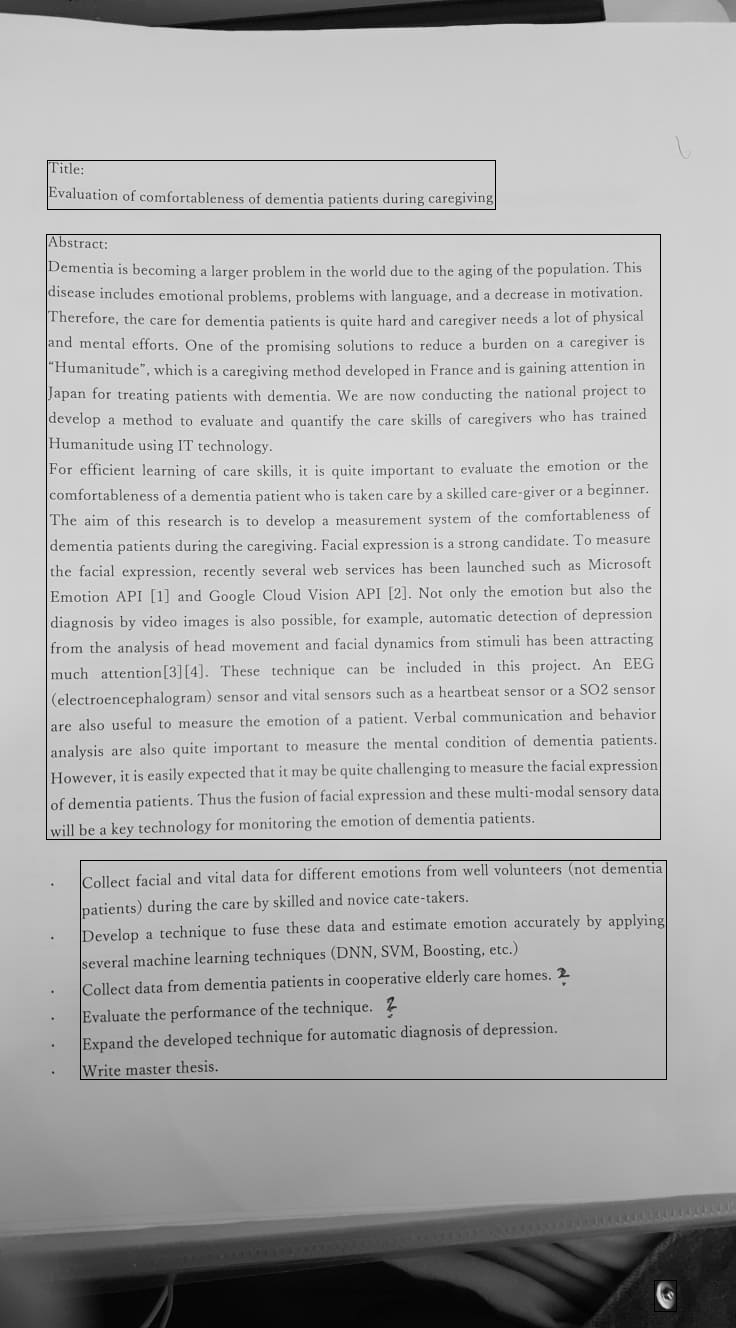
\includegraphics[width=3cm]{res/segment_text2.png}
    \caption{Example 2, Good result on paper}
  \end{subfigure}
  \hspace{5mm}%
  \begin{subfigure}[t]{4cm}
    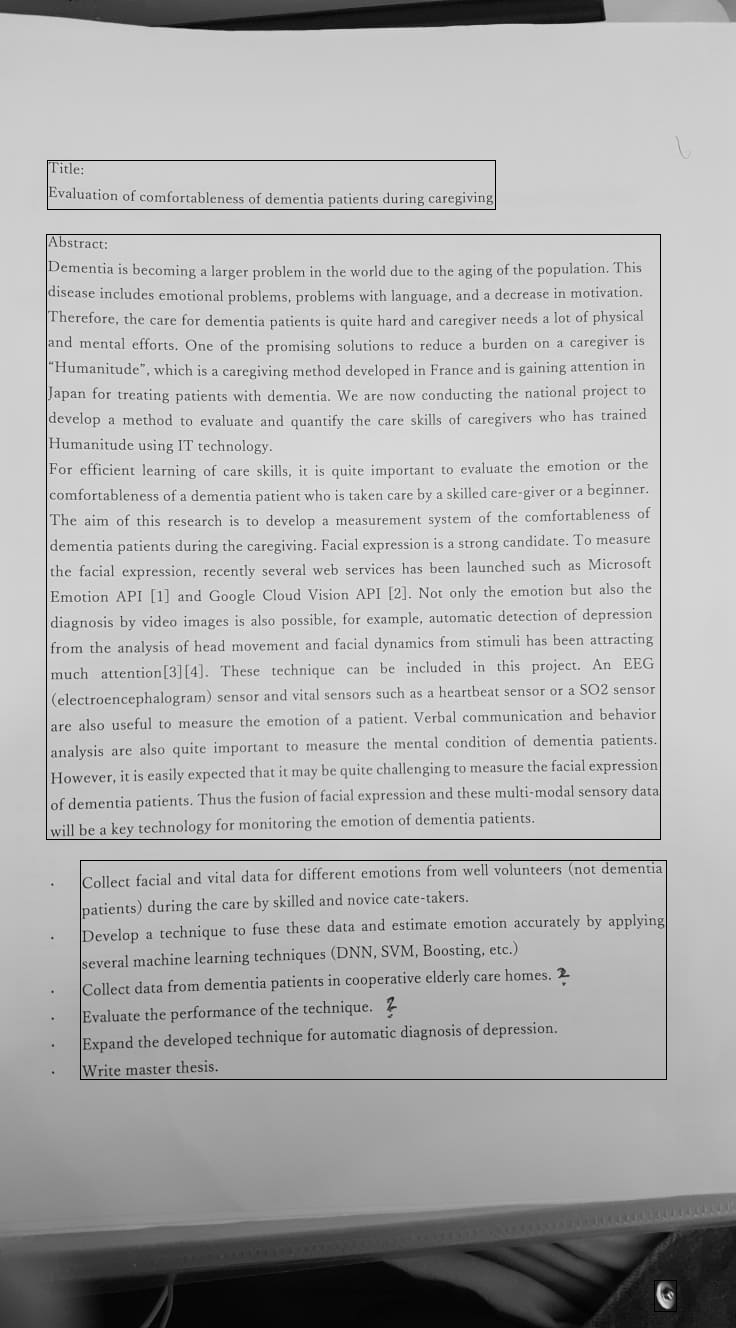
\includegraphics[width=3cm]{res/segment_text3.png}
    \caption{text}
  \end{subfigure}
  \caption{Example 3, Part of the text was not included}
  \label{fig:Text_detection_approaches}
\end{figure}










\section{Component: Preprocessing}
\label{Method:Preprocessing}
\subsection{Description}
Definition of preprocessing; the act of preparing the data for further use,
in our case for classification. \par
After the text segmentation we assume we have an image consisting of white text on black background. What remains for us to do is to segment out each character and format it to the right data type for the classifier. Hence the challenges we will have to solve here are:


\begin{flushleft}
  \textbf{Challenges}
  \begin{itemize}
    \item{Data formatting/casting}
    \begin{itemize}
      \item{The data we want to test a classifier on needs to match the data we trained our classifier with. Hence we need to format our data to the same format as the datasets. No need for a specific approach.}
    \end{itemize}
    \item{Rotated text}
    \begin{itemize}
      \item{Our approach for character segmentation needs text rotated horizontally.}
    \end{itemize}
      \item{Line segmentation}
    \begin{itemize}
      \item{Our approach for character segmentation needs lines as input, as a sequence of lines on top of each other breaks the algorithm.}
    \end{itemize}
      \item{Character segmentation}
    \begin{itemize}
      \item{We need to segment each character because the classifier cannot distinguish several characters from one image.}
    \end{itemize}
  \end{itemize}
\end{flushleft}


\subsection{Find rotation}
\begin{flushleft}
  \textbf{Approach: OpenCV minAreaRect() + CNN solution} \\
  This approach uses \href{https://en.wikipedia.org/wiki/Convex_hull}{convex hull}
  to find the convex hull of the text segments, and then
  \href{https://en.wikipedia.org/wiki/Rotating_calipers}{rotating calipers} to
  find the minimum area rectangle. \par
  One important note here is that the method above operate on binary images, therefor we need to convert our image to binary, possibly using some threshold algorithm. Because we want the convex hull \todo[inline]{(Fjerne dette?) algorithm to find the convex hull} of the text segment. \par
  This method is really good at finding the angles, however it does not solve the problem of rotating the text correctly, Figure~\ref{fig:4angle_rot} illustrates
  this problem. It will only allow us to rotate it along one of the text segments edges. To rotate the text correctly from the result of cv.minAreaRect we decided to try and use another Convolutional neural networks to find if the text was rotated 0, 90, 180 or 270 degrees. For this we had to feed our new network new dataset with rotated images with their corresponding angles. After a quick search on Internet no such dataset was found, so we decided to create it  ourself (We describe our approach later in this document). 

  \begin{enumerate}
    \item \textbf{Binary image}
    For the Convex hull algorithm to work, the text segment and the background needs to be distinguishable. Convert image to a binary image using OpenCV threshold function and possibly bitwise\textunderscore not to flip foreground and background colors.
    \item \textbf{cv.minAreaRect()}
    Feed our newly generated image to cv.minAreaRect with some additional parameters.
    \item \textbf{Custom CNN solution - find correct rotation}
    Now that we have text rotated in one of [0\textdegree, 90\textdegree, 180\textdegree, 270\textdegree], we have several options of finding final rotation angle of current text segment. \todo[inline]{As the above method returns text rotated in one of following angles [0\textdegree, 90\textdegree, 180\textdegree, 270\textdegree], we will use a CNN to determine the which angle it is and then rotate it. We have several options when we use a CNN to find the correct angle.}
    \begin{enumerate}
	\item{Most straightforward would be to find rotation of first character and rotate the whole segment accordingly (fast and naive)}
	\item{Pick N characters and find their rotation, angle with most matches will be our final angle of rotation (somewhat slower (depends on N) but gives us bit more confidence than approach above)}
	\item{Finally we can find angle for each individual character before we try to classify it, gives us the most accuracy but the price is time/computation power. This is the only approach able to successfully recognize this type of text: (find better example)\LaTeX}
	\end{enumerate}
    \end{enumerate}
\end{flushleft}


\subsection{Find line}


\subsection{Find Symbol/Letter Segmentation}
Letter segmentation was similar to Text Segmentation. we added a few steps and removed the morphology part. The additional step was to fill holes in the image, example like 8 and O can give multiple wrong contour. cv2.floodFill was used to solve this problem.
\begin{enumerate}
  \item Do threshold.
  \item Inverse the image since we work on black text on white background.
  \item Fill any holes, cv2.floodFills
  \item FindContours
\end{enumerate}
\subsection{Approach: find contour after Filled holes}
test text alksjdfh alsjkdbfkas


\section{Component: Classification}
\label{Method:Classification}
\begin{flushleft}
  \textbf{Description} \\
  For the classification component there where only 2 approaches we considered,
  Convolutional Neural Network (CNN), the architecture is illustration in
  Figure~\ref{fig:CNN_architecture}, and a Multilayer Perceptron (MLP or Deep
  neural network (DNN)), Figure~\ref{fig:neural_net2}. However the method we
  ended up choosing for the final result is CNN. In
  Section~\ref{sec:Discarded Method:Classification} we explain why we discarded
  the MLP approach. \par
\end{flushleft}

\begin{flushleft}
  \textbf{Convolutional Neural Network} \\
  The basic idea of a CNN is train some number of filters and then
  after the filters are trained, run the image which is now ``filterd'', through
  a fully connected network. The fully connected network will then try and
  classify based on the feature images from the filtering/convolution layers. \par
  \todo[inline]{Bellow we will present, a short description of key points of a CNN, the architecture and variable choices we have made for the CNN.}
\end{flushleft}

\begin{figure}[H]
  \centering
  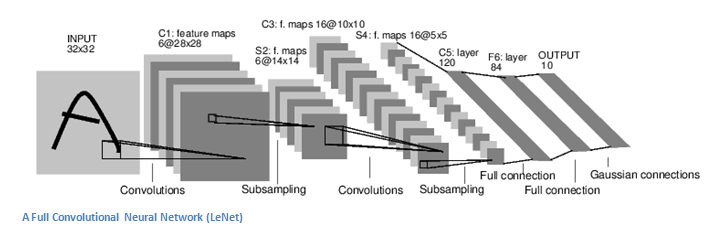
\includegraphics[height=4cm]{res/LeNet.png}
  \caption{Convolutional Neural network \href{https://adeshpande3.github.io/A-Beginner\%27s-Guide-To-Understanding-Convolutional-Neural-Networks/}{Source}}
  \label{fig:CNN_architecture}
\end{figure}

\begin{flushleft}
  \textbf{CNN - Basics} \\
  \begin{itemize}
   \item{Convolutional layer}
   \begin{itemize}
    \item{This layer consists of several filters/kernels that are convolved over the image and based on how many filters one uses, the same amount of feature images are made. The purpose of the filters are to grasp some spatial characteristics of the image, and make it available for further processing.
    The filters here correspond to the weights in the MLP, these are first initialized at random (or with a smart initialization method), then these will be updated as the network is trained. 
First layer filters are able to spot simple geometry like straight or curved lines, but the deeper we dive into networks topology the more complex shapes the filters can recognize. It is not unusual that last layers on large networks can differenciate between faces, animals, objects.\par
    In a CNN we can have arbitrary many convolutional layer and arbitrary many filters at each layer. However just like a regular MLP, increasing the number of layers and or filters; can allow the network to fit the training data arbitrarily well, unfortunately at the cost of processing time, mostly during training, but also during prediction phase.}
   \end{itemize}
   \item{Pooling}
   \begin{itemize}
    \item{The pooling layer allows us to downsize the data. This makes it possible to start with images which are relatively big, and as it's data propagates through the network we downsize it. As for the convolution layer the pooling layer can be used arbitrarily many times in a network.
    Pooling makes our network rotation invariant to minor changes in angle, as outputs max/min value of a (pooling-size) block regardless of where in the block this value is.}
   \end{itemize}
   \item{Fully connected layers (FC)}
   \begin{itemize}
    \item{This layer works basically the same way as the hidden layers in an MLP.
    The output of last convolution layer is then flattened and send to N fully connected layers (also sometimes referenced as dense layer). At the last layer we have same number of outputs as we have classes, just like in regular MLP.}
   \end{itemize}
  \end{itemize}
\end{flushleft}


\section{Component: Datasets}
\label{Method:Datasets}
\subsection{Description}

\begin{flushleft}
  \textbf{Description} \\
  In order to learn our network to distinguish between the characters it needs training. Training is done by feeding images of known objects to the network (labeled data) and telling it how inaccurate it's prediction so that network can adjust it's weights accordingly. This type of training is called supervised training as we guide our network during training process.
For network to get high accuracy of prediction a lot of labeled data is needed. Lucky for us datasets like MNIST exists, more info about it later.
\end{flushleft}

\begin{flushleft}
  \textbf{Limitation - proof-of-concept} \\
  As we have limited us to the digits and English alphabet, we will need labeled data for each of these [0..9] + 36 characters; divided into training, test and validation sets. As the concept of classifying only numbers vs all 36 characters does not differ that much, we will first see if we can solve the OCR problem with just numbers. Therefore we only need a dataset containing numbers at first. After that we can proceed our search for a dataset containing all the characters we need.
\end{flushleft}

\begin{flushleft}
  \textbf{Dataset} \\
  \textbf{MNIST} \\
  This is a dataset containing images of handwritten digits [0-9]. It has a training set of 60.000 examples and a test set of 10.000 examples. Training set is further divided into 55000 examples of actual training set, while 5000 images are treated as validation set (this number can be changed depending which interface we use to access MNIST data).
MNIST dataset is compressed into 4 binary *.gz files, but we dont need to implement any readers/parsers ourself as tensorflow already has two we can choose between.
(ref. reader to http://yann.lecun.com/exdb/mnist/).
\end{flushleft}
\end{document}
